\section{TelcoGAN Model}
In this section, we introduce our TelcoGAN model for Telco missing data completion. The descriptions are separated into four parts. First, we describe the design of TelcoGAN model as well as the interaction of different components. Second, we give the details of relative coordinate space and explore the real-world relationship between connected cells and RSSI. Next, the designs of generator, discriminator and localizer is introduced respectively. Finally, we give TelcoGAN's training process.

\begin{figure}
  \centering
  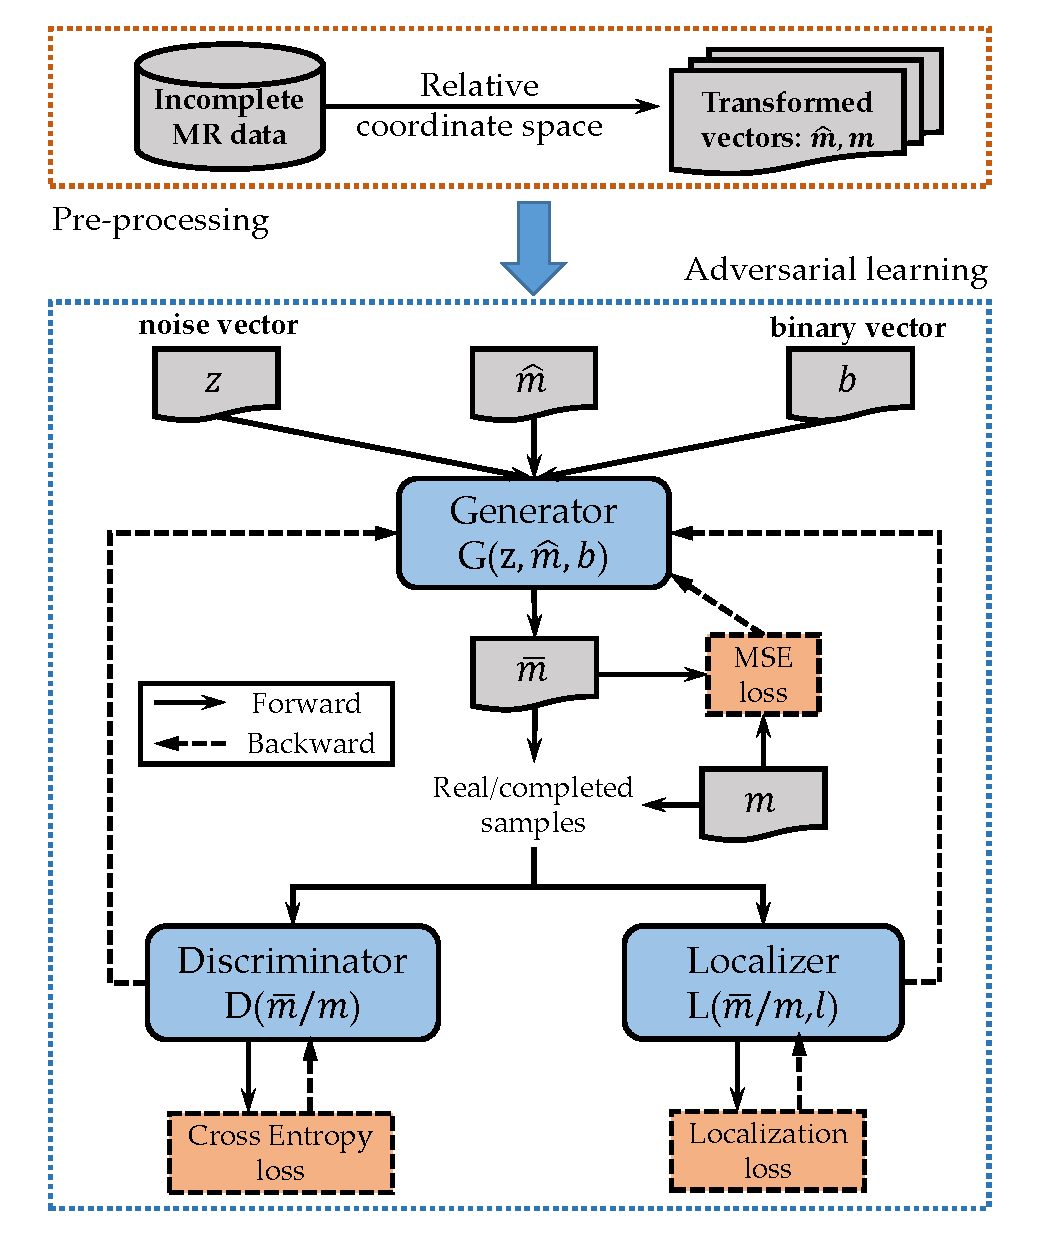
\includegraphics[width=9cm]{pics/framework.pdf}
  \caption{The framework of TelcoGAN}\label{fig:framework}
\end{figure}


\subsection{Overview of TelcoGAN}
The TelcoGAN model consists of pre-processing step and three basic components. The framework of TelcoGAN is illustrated as Fig. \ref{fig:framework}.

In the pre-processing step, due to sparse extensive cell locations in MR data, we propose to apply a relative coordinate space. The sparse global coordinate-based distribution of MR data is transformed into a dense relative coordinate-based distribution. Thus the TelcoGAN model can better capture the internal correlation of cell locations and corresponding RSSI.

The adversarial learning step consists of three interacting components described as follows:

(1) \textbf{Generator} $\bar{\textbf{m}}\sim$ G(\textbf{z},$\hat{\textbf{m}}$, \textbf{b}): The generator takes a random vector, an incomplete MR matrix and corresponding binary vector as input, and generates a completed MR matrix $\bar{\textbf{m}}$ that fools the discriminator as well as makes localizer produce accurate predictions.

(2) \textbf{Discriminator} D($\bar{\textbf{m}}/\textbf{m}$): The discriminator takes either a generated MR sample or a real MR sample as input, and gives each sample the probability over two categories (real/generated).

(3) \textbf{Localizer} L($\bar{\textbf{m}}/\textbf{m}$, $\textbf{l}$): The localizer takes a pair of MR sample and corresponding location label as input. It tries to predict the position of MR sample and minimize the localization loss.

The intuition of how our TelcoGAN model can generate high quality MR data for Telco localization is as follows. The generator tries to recover complete MR data samples based on observed variables to fool the discriminator; The discriminator distinguishes input data samples and computes probability distribution that the samples comes from real data or generated data; The localizer predicts locations of MR samples and produces a score for each sample that reflects its quality. During the adversarial game between the generator and the discriminator, the localizer can guide the optimization towards better data quality by utilizing available location labels. When the training reaches the optimality, the generator will have learnt the mapping from incomplete MR data to complete MR data.

We choose to implement these three components as neural networks. We will discuss their detailed structures for generating complete MR data in the following subsections.


\subsection{Relative Coordinate Space}

\subsection{TelcoGAN Generator}

\subsection{TelcoGAN Discriminator}

\subsection{TelcoGAN Localizer}

\subsection{TelcoGAN Training}
